\documentclass[12pt]{article}
\usepackage[style=apa]{biblatex}  
\addbibresource{Latex_assignmentcor.bib}
\usepackage{graphicx} % Required for inserting images
\usepackage{authblk} % Allows affiliation formatting
\usepackage{tikz}
\usepackage{float} 
\usepackage{booktabs}
  

\usepackage{fancyhdr}
\pagestyle{fancy}
\fancyhf{} 
\fancyhead[L]{AUTONOMIC MARKERS OF DEPRESSION}
\fancyhead[R]{\thepage} 

\begin{document}
\title{The Association Between Autonomic Dysregulation and Depressive Symptoms}
\author{Jenna Glotfelty}
\affil{Department of Psychological Sciences, College of William and Mary}
\date{September 2025}
\maketitle
\begin{center}
\textbf{Keywords:} Depression, Stress, Autonomic Dyresgulation
\end{center}
\section*{Author Note}

I thank Dr. Meghan Smith for her guidance and the lab team for their help with data collection.


\newpage
\section{Introduction}
Depression is a severe mental health condition that hinders the everyday functioning of those afflicted. Diagnostic materials treat depression as a unitary disorder based on observation \parencite{stringaris_editorial_2017}. However, this approach is flawed for several reasons. Depression is heterogeneous, and thus its diagnosis should be based on the presence of a wide range of symptoms. Much of the literature looking at the physiological mechanisms underlying depression is unknown or mixed. The autonomic nervous system fluctuates in response to stress in healthy individuals, and depression is associated with stress \parencite{remes_biological_2021}. Prior research has shown that autonomic dysregulation occurs in depressed individuals, with results suggesting that depression is associated with blunted parasympathetic and heightened sympathetic activation at rest. Despite this, much of the literature emphasizes associations observed during resting periods or baseline conditions, even though fluctuations in these systems in response to stress are of coequal status\parencite{Rottenberg2007RSA}  % for biblatex
. The goal of the present study was to examine which symptoms of depression are associated with autonomic functioning at rest and in response to stress.

\section{Method}
 Participants completed brief daily surveys while actigraphy data were collected for one week. Participants then completed an online survey consisting of various demographic, symptoms (including our measure of depressive symptoms), trait, and stress measures. Participants then returned to the lab to complete session two, approximately one week after the first session. Descriptive statistics of participants can be seen in Table~\ref{tab:descriptives}. In this session, participants were connected to psychophysiological recording equipment, including ECG and EDA sensors. A 5-minute relaxation period followed, with psychophysiological signals recorded while participants watched a neutral video, both while seated and standing. Participants then completed an executive control task (not included in the present study). Participants were then randomized to complete either a stress induction or a control version of the stress induction. Participants then completed another measure of executive control (not included in the present study), which was followed by a 20-minute relaxation period in which participants watched a neutral video. A subset of participants also provided saliva samples throughout the laboratory session (not included in the present study). Finally, a subset of participants completed a follow-up online survey on symptoms (not included in the present study). A pievewise growth curve analysis will be conducted through RStudio to analyze physiological data and depressive symptom interactions. 
 \begin{table}[H]
  \centering
  \caption{Descriptive Statistics by Condition}
  \label{tab:descriptives}
  \resizebox{\textwidth}{!}{
  \begin{tabular}{lcc}
    \toprule
    \textbf{Variable} & \textbf{Stress} M (SD) or \% & \textbf{Control} M (SD) or \% \\
    \midrule
    \textit{Age} & 18.91 (1.40) & 18.94 (1.14) \\
    \midrule
    \textit{Sex} & & \\
    \quad Female & 65.50\% & 66.00\% \\
    \quad Male & 33.80\% & 31.30\% \\
    \quad Other & 0.70\% & 2.80\% \\
    \midrule
    \textit{Race/Ethnicity} & & \\
    \quad White or Caucasian & 43.90\% & 50.70\% \\
    \quad Asian or Asian American & 24.50\% & 18.10\% \\
    \quad Black, African American, or African & 10.10\% & 11.10\% \\
    \quad Latino or Hispanic & 5.00\% & 2.10\% \\
    \quad American Indian, Native American, or Alaskan Native & 0.70\% & 0.00\% \\
    \quad Middle Eastern or Arab & 0.70\% & 0.00\% \\
    \quad Native Hawaiian or Caucasian & 0.00\% & 0.70\% \\
    \quad Multi-Racial & 15.10\% & 16.80\% \\
    \quad Missing & 0.00\% & 0.70\% \\
    \midrule
    \textit{Total $n$} & 139 & 144 \\
    \midrule
    \textit{BDI-II Score} & 11.18 (9.08) & 11.95 (11.15) \\
    \textit{IDAS-II Item 57} & 1.10 (0.39) & 1.26 (0.66) \\
    \bottomrule
  \end{tabular}
  }
\end{table}

 \section{Results}
 We anticipate that participants with higher levels of insomnia, anhedonia, depressed mood, feelings of guilt, and concentration difficulties will predict blunted RSA reactivity during the stress induction. The blunted reactivity we anticipate seeing is illustrated in Figure~\ref{fig:rsa_trajectory}. A more specific example, looking specifically at guilt, can be seen in Figure~\ref{fig:rsaguilt_trajectories}. We predict that participants with higher levels of insomnia, psychomotor retardation, and suicidal ideation will predict hyporeactivity during the stress induction, whereas those experiencing agitation will predict hyperreactivity. 
\begin{figure}[ht]
\centering
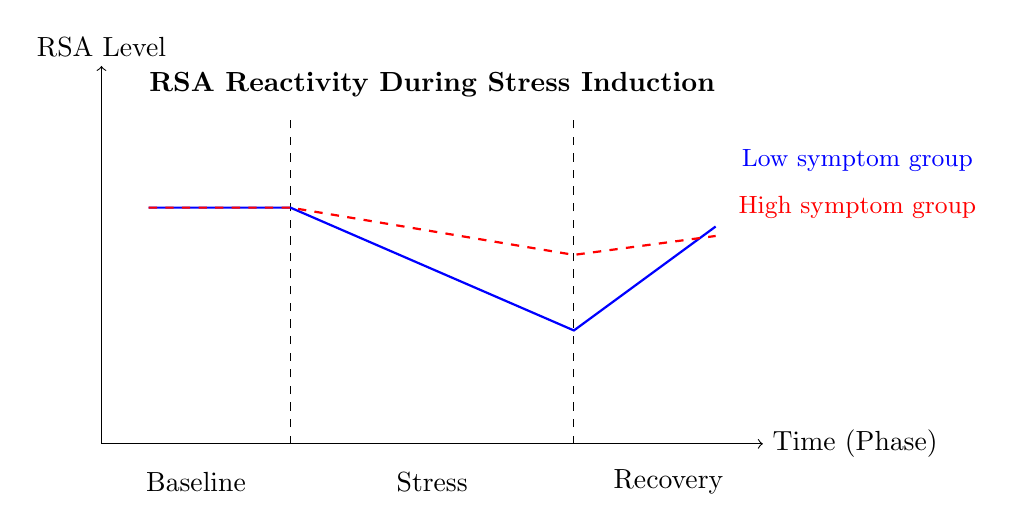
\begin{tikzpicture}[scale=1.2]

  % Axes
  \draw[->] (0,0) -- (7,0) node[right] {Time (Phase)};
  \draw[->] (0,0) -- (0,4) node[above] {RSA Level};

  % Phase markers
  \node at (1,-0.4) {Baseline};
  \node at (3.5,-0.4) {Stress};
  \node at (6,-0.4) {Recovery};

  % Dashed vertical lines for phase boundaries
  \draw[dashed] (2,0) -- (2,3.5);
  \draw[dashed] (5,0) -- (5,3.5);

  % Low symptom group (typical reactivity)
  \draw[thick,blue] (0.5,2.5) -- (2,2.5) -- (5,1.2) -- (6.5,2.3);
  \node[blue] at (8,3) {\small Low symptom group};

  % High symptom group (blunted reactivity)
  \draw[thick,red,dashed] (0.5,2.5) -- (2,2.5) -- (5,2.0) -- (6.5,2.2);
  \node[red] at (8,2.5) {\small High symptom group};

  % Labels
  \node at (3.5,3.8) {\textbf{RSA Reactivity During Stress Induction}};

\end{tikzpicture}
\caption{RSA trajectory across baseline, stress, and recovery phases.}
\label{fig:rsa_trajectory}
\end{figure}

\begin{figure}[H]
  \centering
  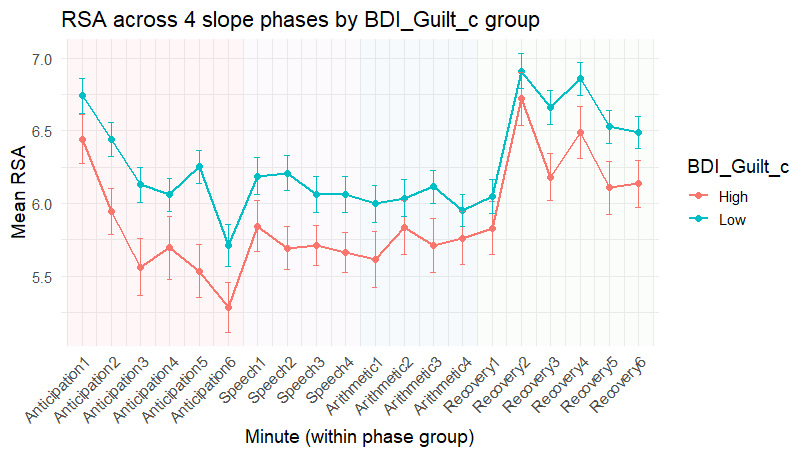
\includegraphics[width=0.8\textwidth]{Guilt.png}
  \caption{Modeled RSA trajectories for participants high and low in guilt.}
  \label{fig:rsaguilt_trajectories}
\end{figure}

 \section{Discussion}
Participants high in melancholic symptoms of depression are more likely to experience vagal withdrawal or blunted reactivity during stress. Participants high in Guilt have lower levels of parasympathetic activation at baseline, indicating dysregulation; however, there is no interaction during stress exposure indicating that this may be a trait-level association rather than a state-dependent response. 
\newpage
\printbibliography
\end{document}
